% !TEX program = xelatex -shell-escape
% !TEX spellcheck = cs_CZ

% Nejprve uvedeme tridu dokumentu s volbami
\documentclass[czech,master,dept460,male,cpp,cpdeclaration]{diploma}
% Dalsi doplnujici baliky maker

\usepackage[backend=biber, style=iso-numeric, alldates=iso]{biblatex} % bibliografie

\usepackage{dcolumn} % sloupce tabulky s ciselnymi hodnotami
\usepackage{subfig} % makra pro "podobrazky" a "podtabulky"
\usepackage{xevlna}
\usepackage{tikz}
\usepackage{mathtools}
\usepackage{amsmath}
\usepackage{amssymb}
\usepackage{bm}
\usepackage{esvect}
\usepackage{pgfplots}
\usepackage{fontspec}
\usepackage{minted}
\usepackage[autostyle=true,czech=quotes]{csquotes} % korektni sazba uvozovek, podpora pro balik biblatex
\usepackage{pifont}
\usepackage{xcolor}
\usepackage{hyperref}

%\setmonofont{[JetBrainsMono-Regular.ttf]}[Contextuals=Alternate,Ligatures=TeX]
%\setmonofont{[Computer Modern]}
\pdfminorversion=6

%Značení normovaného vektoru
%\newcommand{\uvec}[1]{\boldsymbol{\hat{#1}}}

\newcommand{\interval}[1]{\left[{#1}\right]}
\newcommand{\uvec}[1]{\hat{#1}}

\newcommand{\point}{p}

\newcommand{\brdf}{f_r\left(\point,\omega_{o},\omega_{i}\right)}
\newcommand{\normVec}{\uvec{n}}
\newcommand{\inVec}{\omega_{i}}
\newcommand{\outVec}{\omega_{o}}
\newcommand{\refl}{\omega_{r}}
\newcommand{\halfVec}{\uvec{h}}

\newcommand{\outRadiance}{L_o \left( \point,\outVec \right)}
\newcommand{\inRadiance}{L_i \left( \point,\inVec \right)}
\newcommand{\emitRadiance}{L_e \left( \point \right)}
\newcommand{\irradiance}{E \left( \point, \inVec \right)}


\newcommand{\inDotNorm}{\left( \inVec \cdot \normVec \right)}

\newcommand{\randU}{\xi_{1}}
\newcommand{\randV}{\xi_{2}}

\newcommand{\alb}{\rho}
\newcommand{\rough}{\sigma}
\newcommand{\ior}{f_0}

\newcommand{\fromVect}{f}
\newcommand{\toVect}{t}

\pgfplotsset{compat=newest}


\newminted{c++}{
    style=vs,
    frame=lines
}


\newcommand{\true}{\ding{51}}
\newcommand{\false}{\ding{55}}
\newcommand{\undecided}{\dots}

% Zadame pozadovane vstupy pro generovani titulnich stran.
\ThesisAuthor{Richard Zvonek}

\CzechThesisTitle{Interaktivní prohlížeč BRDF funkcí}

\EnglishThesisTitle{Interactive Visualization of BRDF Functions}

\SubmissionDate{30.dubna 2021}

% Pokud nechceme nikomu dekovat makro zapoznamkujeme.
\Thanks{Rád bych na tomto místě poděkoval všem, kteří mi s prací pomohli, protože bez nich by tato práce nevznikla.}

% Zadame cestu a jmeno souboru ci nekolika souboru s digitalizovanou podobou zadani prace.
% Pokud toto makro zapoznamkujeme sazi se stranka s upozornenim.
\ThesisAssignmentImagePath{Figures/Assignment}

% Zadame soubor s digitalizovanou podobou prohlaseni autora zaverecne prace.
% Pokud toto makro zapoznamkujeme sazi se cisty text prohlaseni.
\AuthorDeclarationImageFile{Figures/AuthorDeclaration.jpg}


% Zadame soubor s digitalizovanou podobou souhlasu spolupracujici prav. nebo fyz. osoby.
% Pokud toto makro zapoznamkujeme sazi se cisty text souhlasu.
\CooperatingPersonsDeclarationImageFile{Figures/CoopPersonDeclaration.jpg}

\CzechAbstract{TODO Czech abstract}

\CzechKeywords{TODO Klíčová slova}

\EnglishAbstract{TODO Eng abstract}

\EnglishKeywords{TODO keywords}

\AddAcronym{BRDF}{bidirectional reflectance distribution function}
\AddAcronym{IOR}{index of refraction}
\AddAcronym{PDF}{probability density function}

\addbibresource{main.bib}

% Novy druh tabulkoveho sloupce, ve kterem jsou cisla zarovnana podle desetinne carky
\newcolumntype{d}[1]{D{,}{,}{#1}}


% Zacatek dokumentu
\begin{document}

% Nechame vysazet titulni strany.
\MakeTitlePages
% A nasleduje text zaverecne prace.

\section{Úvod}
TODO
\clearpage
\section{Fotorealistický rendering}
Počítačová grafika se odjakživa snaží svými výsledky co nejvěrněji přiblížit reálnému světu. Fotorealistická grafika je taková, která se tváří jako nerozeznatelná např. od fotografie. Pro fotorealismus je nutné, aby rendering (výpočet geometrie, pozice objektů a osvětlení) co nejpřesněji simuloval fyzikální principy šíření světla. V roce 1986 byl realistický rendering popsán integrální rovnicí popisující přenos světelné energie ve scéně. Renderovací rovnice byla popsána simultánně ve článcích \cite{KajiyaRenderEq} a \cite{ImmelRenderEq}. Kajiya v \cite{KajiyaRenderEq} popisuje různé možnosti řešení integrálu renderovací rovnice, mimo jiné i pomocí Monte Carlo metody, kterou pojmenoval jako path tracing \cite{HainesRayTracingGems2019}. Immel, Cohen a Greenberg v článku \cite{ImmelRenderEq} navrhují řešení renderovací rovnice pomocí metody konečných prvků, kterou pojmenovali jako metodu radiozity. V této práci se budu dále zabývat řešením renderovací rovnice pouze pomocí metody Monte Carlo. \par
Renderovací rovnici lze vyjádřit \hyperref[eq:render]{vzorcem \ref{eq:render}}. Renderovací rovnice bez BRDF členu a bez emisivního členu vyjadřuje intenzitu záření dopadající na danou plochu (viz \hyperref[eq:renderIrradiance]{vzorec \ref{eq:renderIrradiance}})\cite{Dutre2003GICompendum}.

\begin{equation} \label{eq:render}
  \outRadiance = \emitRadiance + \int_{H \left( \point \right)}^{~}\inRadiance \brdf \inDotNorm \,d\inVec
\end{equation}

\begin{equation} \label{eq:renderIrradiance}
  \emitRadiance = \int_{H \left( \point \right)}^{~}\inRadiance \inDotNorm \,d\inVec
\end{equation}

\subsection{Osvětlení}
Jak už bylo zmíněno, realistický rendering se zabývá co nejpřesnější simulací šíření světla ve scéně. V reálném světě je světlo jako takové elektromagnetické záření. Viditelná část světla odpovídá zhruba intervalu $\interval{390;760}nm$ vlnové délky. Při renderingu se často pracuje pouze s geometrickou optikou. Geometrická optika zjednodučuje při šíření světla světelné paprsky na pouhé vektory, zanedbává vlastnosti vycházející z vlnové podstaty světla. Z pohledu počítačové simulace jsou světelné paprsky vyzařovány světelnými zdroji do scény. Objekty ve scéně světelné paprsky pohlcují a nebo odráží. Odraz a pohlcení světla potom definuje, jak výsledný objekt působí. \par
Osvětlení objektů ve scéně je popsáno osvětlovacím modelem. Pokud daný osvětlovací model bere v potaz vliv na osvětlení pouze přímými zdroji světla, jedná se o lokální osvětlovací model. Pokud osvětlovací model bere v potaz i světlo odražené ostatními objekty ve scéně, které samy o sobě žádné světlo nevyzařují, jedná se o globální osvětlovací model. Rozdíl mezi osvětlením lokálním a globálním osvětlovacím modelem je patrný z \hyperref[fig:localVsGlobalIllum]{obrázku \ref{fig:localVsGlobalIllum}}.

\begin{figure}[ht]%
  \centering
  \subfloat[Lokální osvětlovací model]{{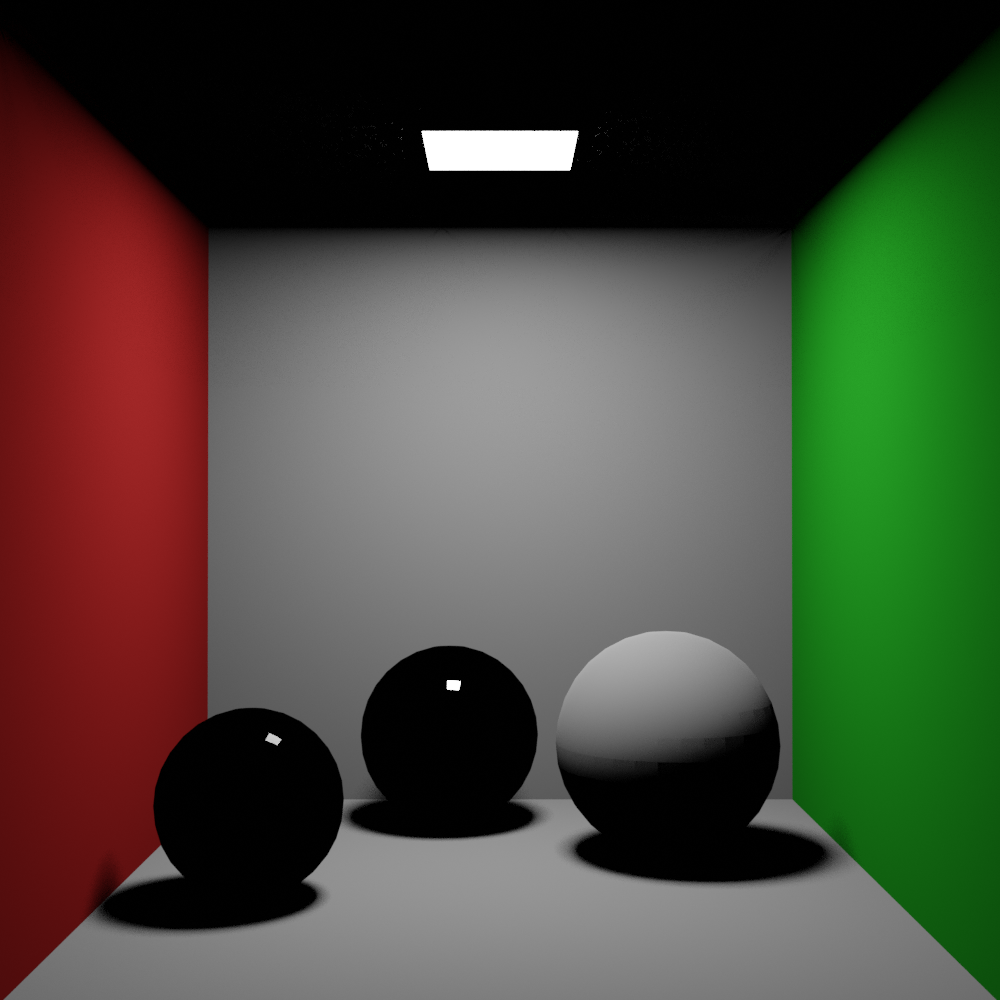
\includegraphics[width=5cm]{Figures/cornelldirect.png} }}%
  \qquad
  \subfloat[Globální osvětlovací model]{{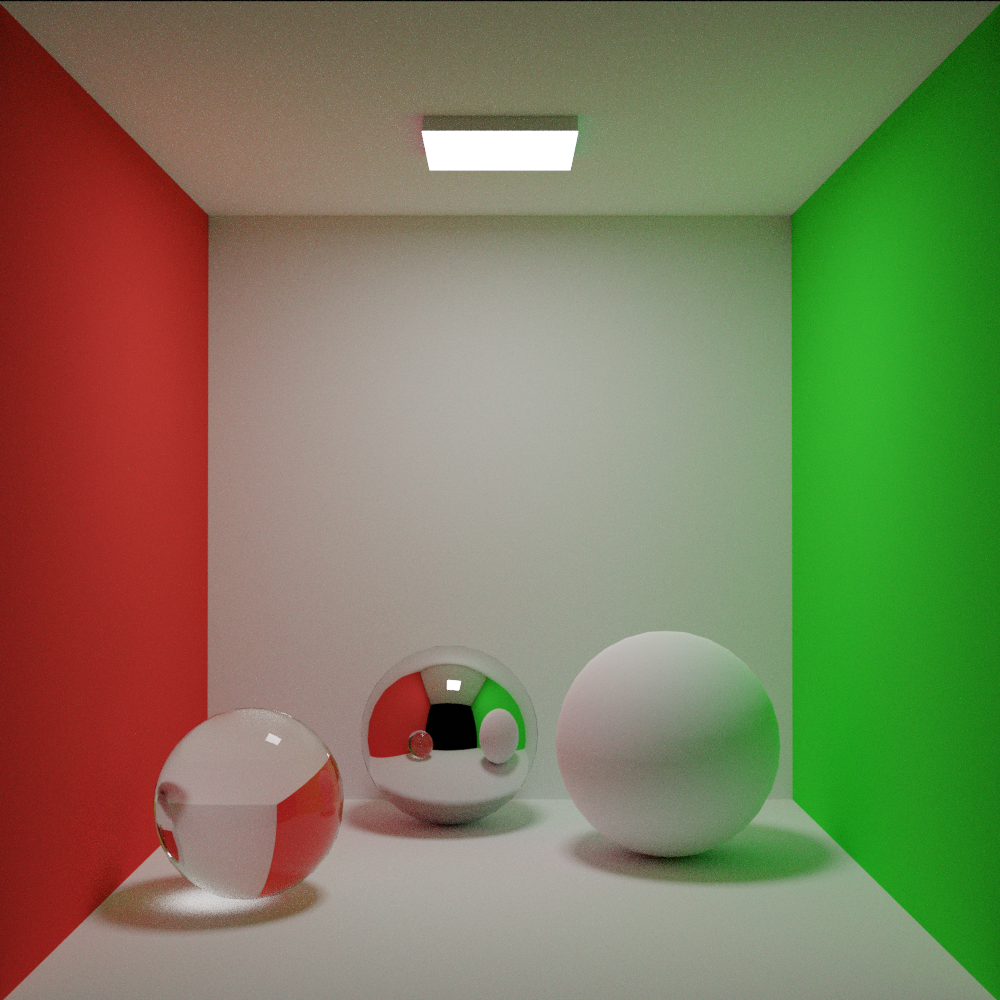
\includegraphics[width=5cm]{Figures/cornellIndirect.png} }}%
  \caption{Srovnání osvětlovacích modelů}%
  \label{fig:localVsGlobalIllum}%
\end{figure}

\subsection{Rendering pomocí metody sledování paprsku}
Při renderingu pomocí klasických metod se postupuje pomocí standardního zobrazovacího řetězce. Postup je ve zkratce následující: Vrcholy tělesa jsou nahrány do GPU, následně se ve fragment shaderu aplikují transformačí matice a matice pro převod z lokálního do globálního prostoru. Následně je provedena rasterizace tělesa. Nakonec je ve fragment shaderu vypočítáno osvětlení tělesa. Standardní zobrazovací řetězec má tu výhodu, že je možné renderovat za běhu programu, v reálném čase. Nevýhodou ovšem je ztráta jisté reálnosti výstupu.\par
Oproti tomu při použití metody sledování paprsku je scéna protnuta s pomyslnou plochou, ze které jsou potom vysílány do scény paprsky ve formě parametrických přímek. Následně se provádí traverzace ve scéně (testování, který objekt ve scéně paprsek protnul). Při protnutí tělesa je možné následně počítat další odrazy paprsků a simulovat tak šíření světla ve scéně. Výhodou použití metody sledování paprsků je možnost velmi reálných výsledků. Nevýhodou je ale vysoká výpočetní náročnost. Výpočet komplexních scén pouze pomocí metod sledování paprsků v reálném čase je komplikovaný problém. V současné době je možná hardwarová akcelerace na grafických kartách. Pro urychlení výpočtu jsou také používány hluboké neuronové sítě (např. technologie Nvidia DLSS). Je možné provádět výpočet pro nižší rozlišení a následně provést upscaling (zvýšení rozlišení). Neuronová síť je schopná dopočítat chybějící data. Výsledkem je dle Nvidia obraz svou kvalitou srovnatelný s výpočtem rovnou ve vyšším rozlišení.

\subsection{Řešení renderovací rovnice pomocí metody Monte Carlo}
Analytické řešení renderovací rovnice je téměř nemožné kvůli obrovskému množství vlivů na výsledném integrálu. Z matematického hlediska existuje více způsobů, jak řešit integrály. Monte Carlo se opírá o tezi z teorie pravděpodobnosti, že průměr velkého počtu náhodných veličin se přiblíží střední hodnotě. Řešení renderovací rovnice pomocí metody Monte Carlo navrhuje Kajiya v \cite{KajiyaRenderEq}. \par
Monte Carlo je stochastická metoda, v matematice často využívaná pro řešení složitějších integrálů. Metoda je založena na generování náhodných jevů, které jsou následně použity pro určení střední hodnoty výsledku. Pro řešení renderovací rovnice jsou typicky generovány náhodné směry odrazu světla. Výsledný obraz je poté tvořen průměrem určitého počtu vzorků. Typicky se u výsledných obrázků vytvořených pomocí path tracingu uvádí počet vzorků na pixel. Se zvyšujícím se počtem vzorků na pixel typicky stoupá ostrost a přesnost výsledného obrazu. S nízkým počtem vzorků je typicky obraz zatížen šumem (viz zrovnání na \hyperref[fig:samplesPpxCOmparison]{obrázku \ref{fig:samplesPpxComparison}}).

\begin{figure}[ht]%
  \centering
  \subfloat[1 vzorek na pixel]{{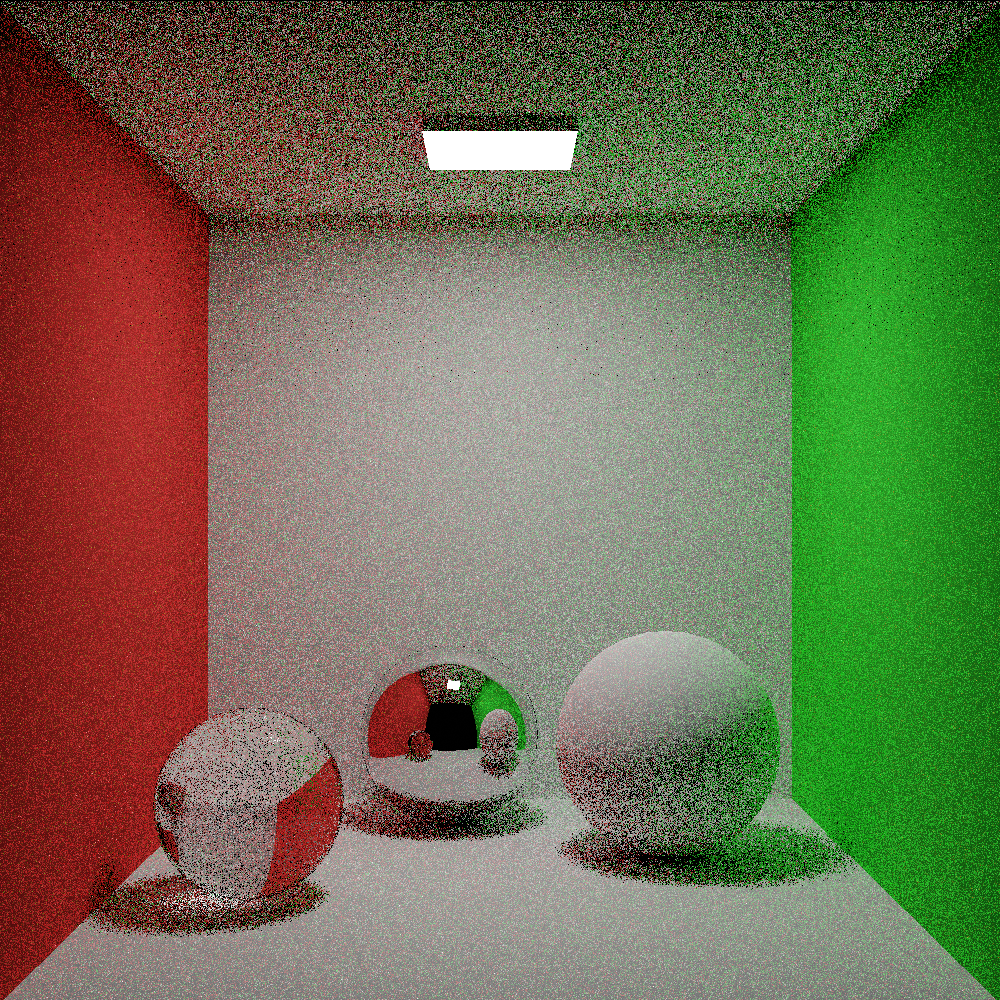
\includegraphics[width=5cm]{Figures/cornell1ppx.png} }}%
  \qquad
  \subfloat[4 vzorky na pixel]{{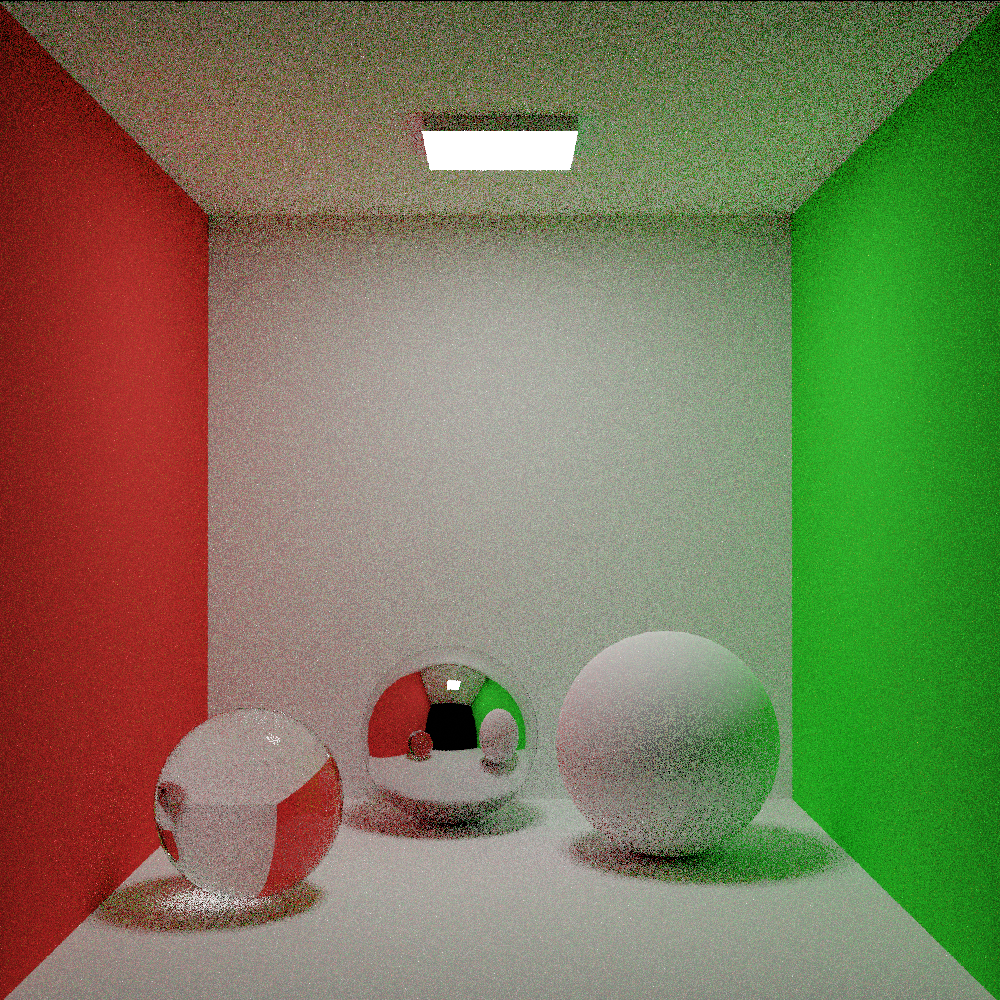
\includegraphics[width=5cm]{Figures/cornell4ppx.png} }}%
  \qquad
  \subfloat[16 vzorků na pixel]{{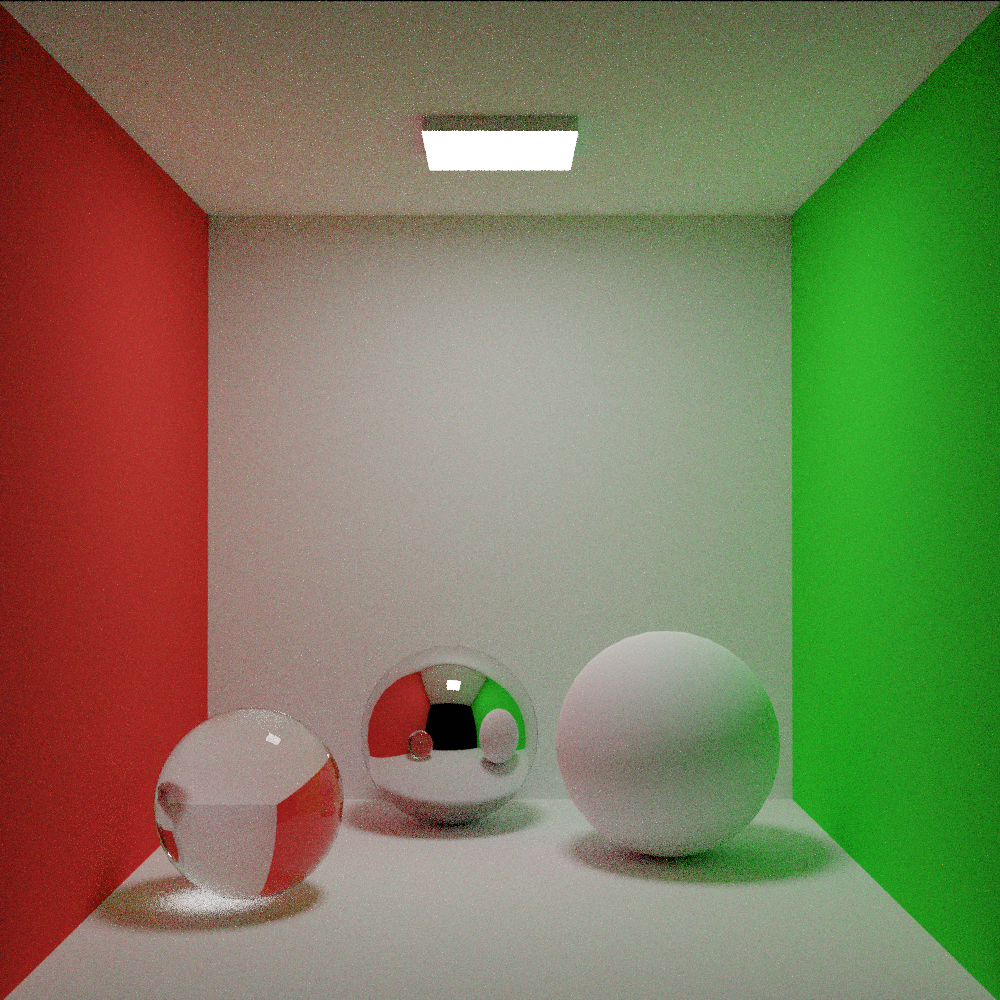
\includegraphics[width=5cm]{Figures/cornell16ppx.png} }}%
  \qquad
  \subfloat[64 vzorků na pixel]{{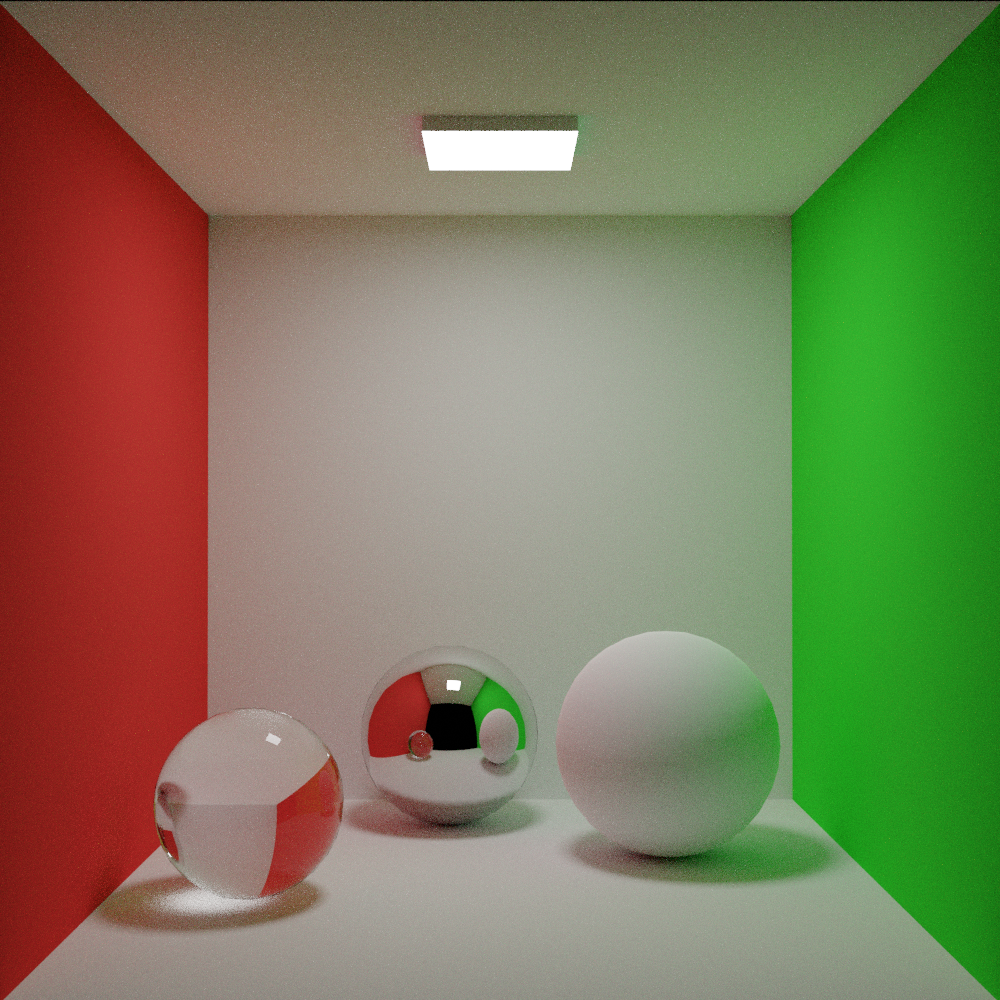
\includegraphics[width=5cm]{Figures/cornell64ppx.png} }}%
  \caption{Srovnání výsledných obrázků podle počtu vzorků na pixel}%
  \label{fig:samplesPpxComparison}%
\end{figure}





\textit{TODO, pojmy:  realistický rendering, path tracing, renderovací rovnice, monte carlo, světlo, osvětlovací model (lokální, globální iluminace), osvětlení pomocí HDR}.

\clearpage
\section{BRDF}
BRDF je matematická funkce, která definuje pro daný materiál odrazivost povrchu. Určuje pro každý bod tělesa distribuci odrazu světla. Na \hyperref[fig:brdf2D]{obrázku \ref{fig:brdf2D}} je znázorněn základní princip BRDF funkce. Vektor \(\normVec\) je normála povrchu, \(\inVec\) značí směr ke světelnému zdroji, \(\outVec\) značí směr k pozorovateli (ke kameře). BRDF je definována pro dvojici vektorů  \(\inVec\) a \(\outVec\) v daném bodě \(p\) pomocí \hyperref[eq:brdf]{vzorce \ref{eq:brdf}}.
% Pbrt strana 350

\begin{equation} \label{eq:brdf}
  \brdf = \frac{d\outRadiance}{d\irradiance} = \frac{d\outRadiance}{\inRadiance \inDotNorm d\inVec}
\end{equation}

Je žádoucí, aby BRDF funkce splňovaly některá základní pravidla. Je důležitá  fyzikální přesnost BRDF funkce, pro kterou musí být musí být splněny následující podmínky \cite{PHARR2017313}:
\begin{enumerate}
  % 10.3 Reciprocity 
  \item Princip vzájemnosti (Helmholtzův princip reciprocity, \cite{hapke_2012}) - Pro všechny dvojice \(\inVec\) a \(\outVec\) platí: \(\brdf = f_r\left(p,\inVec,\outVec\right)\)
  \item Princip zachování energie - Celková energie odraženého světla nemůže být vyšší, než energie vstupního světla
  \item BRDF musí mít vždy nezáporný výsledek
\end{enumerate}
\begin{figure}[ht!]
  \centering
  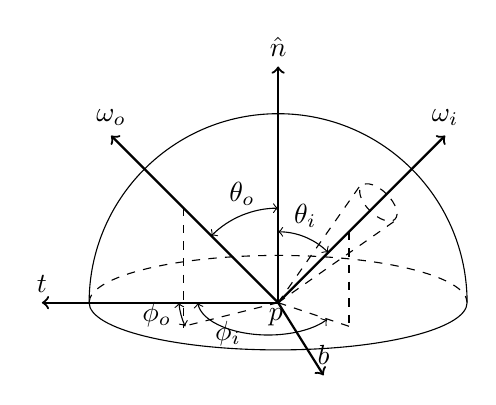
\begin{tikzpicture}[scale=0.6]
    % base circle
    \draw (-4,0) arc (180:360:4 and 1);
    \draw [dashed] (-4,0) arc (180:0:4 and 1);
    % hemisphere
    \draw (-4,0) arc (180:0:4 and 4);

    \draw [thick, ->] (0,0) -- ++(-5,0) node [at end, above] () {\(\vv{t}\)};
    \draw [thick, ->] (0,0) -- ++(135:5cm) node [at end, above] () {\(\outVec\)};
    % y
    \draw [thick, thick, ->] (0,0) -- ++(0,5) node [at end, above] () {\(\normVec\)};
    % z
    \draw [thick, ->] (0,0,0) -- ++(0,-2.5,-2.5) node [at end, above] () {\(\vv{b}\)};
    % lines spanning angle alpha
    \draw [thick, ->] (0,0) -- ++(45:5cm) node [at end, above] () {\(\inVec\)};

    \draw [thin, dashed] (0,0) -- ++(55:3cm);
    \draw [thin, dashed] (0,0) -- ++(35:3cm);

    \draw[thin, dashed, rotate=45] (3,0) ellipse (0.25cm and 0.5cm);

    \draw [thin, <->] (0,0) ++(90:1.5cm) arc (90:45:1.5cm) node [midway, above] () {\(\theta_i \)};

    \draw [thin, dashed] (1.5,1.5) -- ++(0,-2);
    \draw [thin, dashed] (0,0) -- ++(1.5,-0.5);

    \draw [thin, dashed] (-2,2) -- ++(0,-2.53);
    \draw [thin, dashed] (0,0) -- ++(-2,-0.5);

    \draw [thin, <->] (0,0) ++(180:2.1cm) arc (185:205:1.5cm) node [midway, left] () {\(\phi_o\)};

    \draw [thin, <->] (0,0) ++(180:1.7cm) arc (185:326:1.5cm and 0.75cm) node [midway, left] () {\(\phi_i \)};

    \draw [thin, <->] (0,0) ++(90:2cm) arc (90:135:2cm) node [midway, above] () {\(\theta_o\)};


    \draw (-0.05,-0.3) node () {\(p\)};
  \end{tikzpicture}
  \caption{Základní vizualizace BRDF funkce}
  \label{fig:brdf2D}
\end{figure}

\subsection{Přehled BRDF funkcí} \label{sec:brdffunctions}
Následující odstavce se zabývají detailním popisem a vlastnostmi jednotlivých BRDF funkcí. Budou zde vyjmenovány pouze ty BRDF funkce, které byly implementovány v praktické části této diplomové práce. \\
Pro rychlý přehled vlastností jednotlivých BRDF funkcí je možné využít \hyperref[tab:brdfProperties]{tabulku \ref{tab:brdfProperties}} (převzato z \cite{BRDFOverview}, zkráceno, doplněno).

\begin{table}[ht]
  \centering
  \begin{tabular}{r|lllllll}
    \hline
    BRDF model          & \rotatebox{90}{Physical} & \rotatebox{90}{Plausible} & \rotatebox{90}{Fresnel Eq}. & \rotatebox{90}{Anisotropic} & \rotatebox{90}{Sampling} & \rotatebox{90}{Rel. cost (cycles)} & \rotatebox{90}{Material type} \\
    \hline
    Ideal reflection    & \true                    & \true                     & \false                      & \false                      & \true                    & \(x\)                              & Mirror, perfect spec.         \\
    Lambert             & \true                    & \true                     & \false                      & \false                      & \true                    & \(x\)                              & Perfect diffuse               \\
    Phong               & \false                   & \false                    & \false                      & \false                      & \true                    & \undecided                         & Rough surf.                   \\
    Blinn-Phong         & \false                   & \false                    & \false                      & \false                      & \true                    & \(9.18x\)                          & Rough surf.                   \\
    Phys. correct Phong & \false                   & \true                     & \false                      & \false                      & \true                    & \undecided                         & Rough surf.                   \\
    Torrance-Sparrow    & \true                    & \false                    & \true                       & \true                       & \false                   & \undecided                         & Rough surf.                   \\
    Cook-Torrance       & \true                    & \true                     & \true                       & \false                      & \false                   & \(16.9x\)                          & Metal, plastic                \\
    Oren-Nayar          & \true                    & \true                     & \false                      & \false                      & \true                    & \(10.98x\)                         & Matte, dirty                  \\
    \hline
  \end{tabular}
  \caption{Stručný přehled implementovaných BRDF funkcí}
  \label{tab:brdfProperties}
\end{table}

\subsubsection{Lambert} \label{sec:Lambert}
Lambertovo BRDF (Lambertovský povrch) se řadí mezi analytické modely BRDF. Popisuje ideálně matné povrchy, které odráží příchozí světlo do všech směrů rovnoměrně se stejnou pravděpodobností, nehledě na příchozí směr paprsku. Jedná se o nejjednodušší BRDF funkci, je definována \hyperref[eq:lambertBRDF]{vztahem \ref{eq:lambertBRDF}} \cite{Koppal2014}.
%COmputer vision reference guide katushi, page 675 - Lambertian Reflectance
\begin{equation} \label{eq:lambertBRDF}
  \brdf = \frac{\alb}{\pi} = konst.
\end{equation}
\(\alb\) ve \hyperref[eq:lambertBRDF]{vztahu \ref{eq:lambertBRDF}} vyjadřuje poměr mezi pohlceným a odraženým světlem. Tato veličina je také odborně nazývána pojmem albedo. Dělení konstantou \(\pi\) zajišťuje platnost zákona zachování energie. Díky nezávislosti na směru vstupního paprsku je také splněna reciprocita.

\subsubsection{Phong} \label{sec:Phong}
Phongovo BRDF vychází z Phongova osvětlovacího modelu, řadí se mezi analytické modely BRDF a používá se pro lesklé povrchy. Původní model je definován \hyperref[eq:phongBRDF]{vzorcem \ref{eq:phongBRDF}} \cite{Phong1975}
\begin{equation} \label{eq:phongBRDF}
  \brdf = k_s(\refl\cdot\outVec)^n
\end{equation}

Upravený, také často využívaný Blinn-Phong model je definován \hyperref[eq:blinnBRDF]{vzorcem \ref{eq:blinnBRDF}} \cite{BlinnPhong1977}. Výhodou upraveného Blinn-Phongova modelu oproti klasickému Phongovu modelu je hladší přechod odlesku světla.

\begin{equation} \label{eq:blinnBRDF}
  \brdf = k_s(\normVec\cdot\halfVec)^n
\end{equation}

Jak Phong, tak Blinn-Phong modely nejsou fyzikálně přesné - nesplňují zákon zachování energie, ani zákon reciprocity \cite{BRDFOverview}. Phongovo BRDF je možné dále upravit, aby byly splněny pravidla pro fyzikální korektnost. Fyzikálně korektní Phongovo BRDF je definováno \hyperref[eq:phongPhysicalBRDF]{vzorcem \ref{eq:phongPhysicalBRDF}}. Pro fyzikální korektnost této varianty Phongova BRDF je potřeba dodržet \(k_d + k_s \leq 1\) \cite{LaFortunePhongBRDF}.

\begin{equation} \label{eq:phongPhysicalBRDF}
  \brdf = \frac{k_d}{\pi} +
  \frac{k_s\left(n+2\right)}{2\pi}\left(\cos\theta_r\right)^n
\end{equation}

\subsubsection{Torrance-Sparrow} \label{sec:torrancesparrow}
Torrance-Sparrow BRDF patří mezi fyzikální modely a je považován za jeden s nejúplnějších modelů \cite{BRDFOverview}. Mimo jiné je např. schopen simulovat odlesk polarizovaného světla. Tento model simuluje mikroploškové materiály a pomocí parametru roughness (drsnost) simuluje mikroskopické nerovnosti materiálu. Orientace mikroskopických nerovností je v materiálu náhodná. Vyšší hodnota drsnosti materiálu snižuje lesklost materiálu. Torrance-Sparrow brdf funkce je definována \hyperref[eq:TorranceSparrow]{vzorcem \ref{eq:TorranceSparrow}}. \par
Pro výpočet se používá distribuční funkce \(D\), která generuje rozložení normál mikroplošek. V této konkrétní implementaci je použita Beckmannova distribuční funkce (viz \hyperref[eq:beckDistr]{vzorec \ref{eq:beckDistr}}). Beckmannova distribuční funkce pracuje s normálou mikroplošky (kolem které se generuje rozložení) a hodnotou drsnosti materiálu. Jako normála mikroplošky je použit poloviční vektor mezi pohledovým a světelným vektorem (viz \hyperref[sec:Phong]{\ref{sec:Phong} Phong}) z důvodu, že mikroploška perfektně odráží světlo právě v případě, kdy je orientovaná podél polovičního vektoru \cite{PHARR2017507}. \par
Dále se počítá poměr odraženého světla a lomeného světla \(F\) pomocí Fresnelových vzorců. Pro výpočet je použita Schlickova aproximace (viz \hyperref[eq:schlickFresnel]{vzorec \ref{eq:schlickFresnel}}) \cite{SchlickFresnel}. \par
Poslední část pro výpočet je koeficient geometrického útlumu \(G\), která vyjadřuje zakrytí mikroplošek při odrazu světla (viz \hyperref[eq:geomAtatenuation]{vzorec \ref{eq:geomAtatenuation}}) \cite{BRDFOverview}.


\begin{eqnarray}
  \brdf & = & \frac{k_d}{\pi} + \frac{k_s D(\halfVec,\rough) F(\outVec) G(\outVec,\inVec)}{4\pi (\normVec \cdot \inVec)}\label{eq:TorranceSparrow}\\
  D(\halfVec,\rough) & = & \frac{e^{\left(\frac{(\normVec\cdot \halfVec)^2-1}{\rough^2(\normVec \cdot \halfVec)^2}\right)}}{\rough^2(\normVec\cdot \halfVec)^2}\label{eq:beckDistr}\\
  F(\outVec) & \approx & R(\theta) = \ior + (1-\ior)(1-\cos\theta)^5\label{eq:schlickFresnel}\\
  G(\outVec,\inVec) & = & \min \left( 1, \frac{2 ( \normVec \cdot \halfVec ) ( \normVec \cdot \outVec )
    }{ ( \outVec \cdot \halfVec ) },\frac{ 2 ( \normVec \cdot \halfVec ) ( \normVec \cdot \inVec ) }{ ( \outVec \cdot \halfVec ) } \right) \label{eq:geomAtatenuation}
\end{eqnarray}
\subsubsection{Cook-Torrance}
Cook-Torrance BRDF rozšiřuje mikroploškové BRDF s myšlenkou, že pouze mikroplošky orientované podél vektoru \(\halfVec\) mají vliv na výsledném odrazu světla. Odrazová složka výsledného obrazu využívá pro výpočet opět funkce \(F, D, G\) (viz \hyperref[sec:torrancesparrow]{\ref{sec:torrancesparrow} Torrance-Sparrow}). Cook-Torrance BRDF se vypočítá podle \hyperref[eq:CookTorrance]{vzorce \ref{eq:CookTorrance}} \cite{CookTorranceBRDF}. Nevýhodou této BRDF funkce je nesplnění fyzikální přesnosti z důvodu nesplnění zákona zachování energie pro některé \(\left(\outVec,\inVec\right)\) \cite{BRDFOverview}.

\begin{equation} \label{eq:CookTorrance}
  \brdf  = \frac{F(\outVec)}{\pi} \frac{D(\halfVec,\rough)}{(\normVec\cdot\inVec)} \frac{G(\outVec,\inVec)}{(\normVec\cdot\outVec)}
\end{equation}

\subsubsection{Oren-Nayar}
Oren-Nayar BRDF popisuje Lambertovské difusivní materiály. Oproti Lambertovu BRDF (\hyperref[sec:Lambert]{viz \ref{sec:Lambert} Lambert}) pracuje s mikroploškami, které ale na rozdíl od mikroplošek popisovaných např. \hyperref[sec:torrancesparrow]{Torrance-Sparrow} modelem nejsou odrazivé, ale difuzivní. Oren-Nayar bere v úvahu odrazy světla mezi jednotlivými mikroploškami s limitovaným maximálním počtem odrazů mezi dvojicí mikroplošek. Pro generování distribuce orientace mikroplošek je použito Gaussovo rozdělení \cite{OrenNayar} \cite{BRDFOverview}. Oren-Nayar BRDF je definováno \hyperref[eq:OrenNayar]{vzorcem \ref{eq:OrenNayar}}

\newcommand{\cosphiri}{\cos\left(\phi_r-\phi_i\right)}

\begin{eqnarray}
  \alpha & = & \max(\theta_i , \theta_o) = \max(\arccos(\normVec\cdot\inVec), \arccos(\normVec\cdot\outVec)) \nonumber \\
  \beta & = & \min(\theta_i , \theta_o) = \min(\arccos(\normVec\cdot\inVec), \arccos(\normVec\cdot\outVec)) \nonumber \\
  \cosphiri & = & \widehat{\left( \inVec - \normVec(\normVec\cdot\inVec) \right)} \cdot \widehat{\left( \outVec - \normVec(\normVec\cdot\outVec)  \right)} \nonumber \\
  C_1 & = & 1-0.5\frac{\rough^2}{\rough^2 + 0.33} \nonumber \\
  C_2 & = & \left\{\begin{matrix*}[l] 0.45\frac{\rough^2}{\rough^2+0.09}\sin\alpha & \cosphiri \geq 0\\ 0.45\frac{\rough^2}{\rough^2+0.09}\left(\sin\alpha-\left(\frac{2\beta}{\pi}\right)^3\right) & jinak \end{matrix*}\right. \nonumber \\
  C_3 & = & 0.125\left(\frac{\rough^2}{\rough^2 + 0.009}\right)\left(\frac{4\alpha\beta}{\pi^2}\right)^2 \nonumber \\
  L^{1}_{r} & = & \frac{\alb}{\pi}\left[C_1 + \cosphiri C_2\tan\beta + \left( 1-\left | \cosphiri  \right | \right)C_3\tan \left(\frac{\alpha+\beta}{2}\right)\right] \nonumber \\
  L^{2}_{r} & = & 0.17\frac{\alb^2}{\pi}\frac{\rough^2}{\rough^2+0.13}\left[1 - \cosphiri  \left(\frac{2\beta}{\pi}\right)^2 \right] \nonumber \\
  \brdf & = & L^{1}_{r} + L^{2}_{r} \label{eq:OrenNayar}
\end{eqnarray}

\clearpage
\section{Vizualizační aplikace}
Aplikace jako taková umožňuje zobrazit BRDF funkce popsané v kapitole \hyperref[sec:brdffunctions]{\ref{sec:brdffunctions} Přehled BRDF funkcí}. Důležitým prvkem je také interaktivita, kdy je možné měnit jednotlivé parametry BRDF funkcí. Kromě samotných BRDF funkcí aplikace umožňuje zobrazit i metody pro vzorkování funkcí (toto téma je dále rozebráno v kapitole \hyperref[sec:reduction]{\ref{sec:reduction} Redukce variance, optimalizace Monte carlo}), kdy je možné přepínat mezi jednotlivými BRDF funkcemi a vzorkovacími funkcemi. Je tedy možné demonstrovat důležitost správného výběru vzorkovací funkce k vybrané BRDF funkci. Pro doplnění funkcionality obsahuje aplikace také možnost pro uložení snímku aktuální vizualizace BRDF ve vysokém rozlišení. \par
Poslední funkcionalitou je interaktivní okno s jednoduchou scénou, která je renderována s použitím aktuálně vybrané BRDF funkce. Pro jednoduchost je renderován model koule, která je popsána analyticky. Tato testovací scéna je primárně osvětlena HDR obrazem, ale aplikace také umožňuje osvětlit scénu konstantním jasem. Tímto nastavením je simulována situace, kdy na objekt dopadá ze všech směrů stejné množství světla. Takto osvětlená scéna je známa jako tzv. Furnace test a slouží pro kontrolu fyzikální korektnosti BRDF funkce.\par
Následující odstavce se zabývají konkrétními detaily implementace a popisem technických řešení použitých pro jednotlivé funkce implementované vizualizační aplikace.

\subsection{Existující řešení}
Existuje množství aplikací řešících podobnou tematiku. V zásadě lze tyto aplikace rozdělit do dvou kategorií:
\begin{enumerate}
  \item Aplikace pro zobrazení BRDF funkcí
  \item Aplikace pro návrh BRDF funkcí
\end{enumerate}
Aplikace vytvořená v této práci spadá do první kategorie, primárně se zabývá pouze zobrazováním. V následujících odstavcích jsou popsány vybrané aplikace z obou kategorií.
\subsubsection{Aplikace pro zobrazení BRDF funkcí}

\subsubsection{Aplikace pro návrh BRDF funkcí}
Ve článku \cite{Fors2009BRDFLabAG} je popsána aplikace pro vizualizaci BRDF funkcí zadaných analyticky, pomocí nameřěných dat, nebo pomocí dat získaných simulací. Také je možné vytvořit BRDF funkce kombinací analyticky zadaných, předpřipravených laloků. Aplikace také umožňuje vizualizaci finálního renderu s použitím BRDF funkce. Aplikace je distribuována jako open-source, pro GUI je použita knihovna QT, pro rendering je použita knihovna Ogre3D.
\par

\subsection{Vizualizace BRDF}
Při implementaci jsem se chtěl co nejvíce přiblížit standardním referenčním obrázkům popisujícím princip BRDF funkcí (viz \hyperref[fig:brdf2D]{obrázek \ref{fig:brdf2D}}). Výsledná vizualizace znázorňuje  pro daný vstupní směr všechny možné výstupní směry, do kterých se světlo odráží. Této vizualizace se dá jednoduše dosáhnout tak, že se vygeneruje jednotková hemisféra a jednotlivé body na hemisféře jsou posunuty o hodnotu BRDF funkce pro daný vstupní a výstupní směr. Každý bod na hemisféře zvýrazňuje výstupní směr, vzdálenost bodu od středu (délka vektoru) zvýrazňuje hodnotu BRDF funkce. \par
Pro vizualizaci jsem se rozhodl vygenerovat jednotkovou polokouli a jednotlivé body polokoule upravit v OpenGL Vertex shaderu. Při generování polokoule jsem narazil na problém, kdy pro vizualizaci bylo potřeba mít co nejrovnoměrněji rozložené polygony, ideálně všechny s podobnou velikostí. Rozhodl jsem se tedy negenerovat UV kouli, ale geodetický mnohostěn (srovnání na \hyperref[fig:spheresComparison]{obrázku \ref{fig:spheresComparison}}), který je tvořen rovnostrannými trojúhelníky.  \par

\begin{figure}[ht]
  \centering
  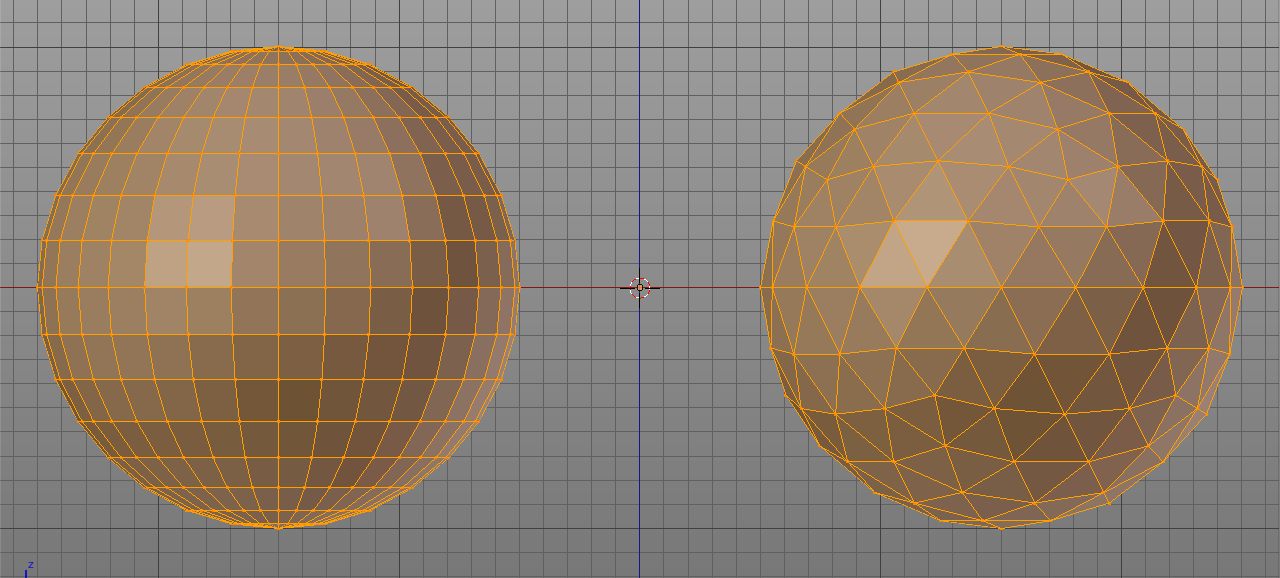
\includegraphics[width=10cm]{Figures/IcosphereUVSphereComparison.png}
  \caption{Srovnání UV koule a geodetického mnohostěnu, z \cite{tan_2019}}
  \label{fig:spheresComparison}
\end{figure}
Pro zjednodušení implementace jsem vycházel z kódu pro dvacetistěn \cite{OpenGLSphere}, jehož trojúhelníkové stěny jsem dále rekurzivně dělil. Počet rekurzivních dělení určuje rozlišení výsledné vizualizace, s vyšším počtem dělení se zvyšuje rozlišení. Postup generování hemisféry použité pro vykreslení BRDF funkcí je zobrazen na \hyperref[fig:hemisfera]{obrázku \ref{fig:hemisfera}}.\par

\begin{figure}[ht]%
  \centering
  \subfloat[Dvacetistěn \label{fig:icasehedron}]{{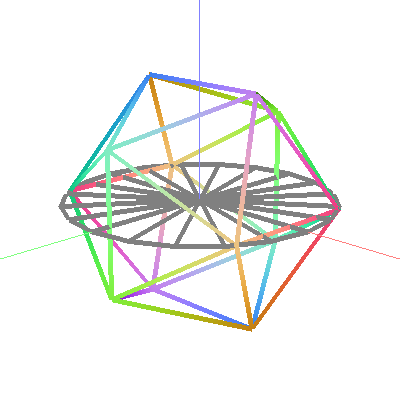
\includegraphics[width=5cm]{Figures/icosphere.png} }}%
  \qquad
  \subfloat[Poloviční dvacetistěn \label{fig:halficasehedron}]{{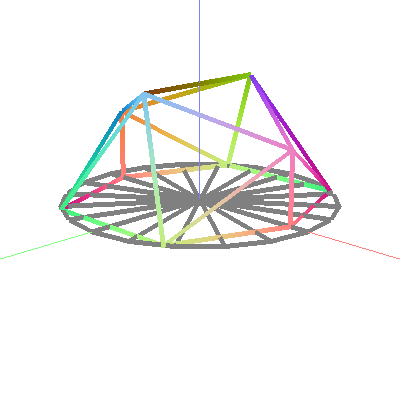
\includegraphics[width=5cm]{Figures/halficosphere.png} }}%
  \qquad
  \subfloat[Poloviční dvacetistěn, \(1\times\) rozdělené polygony \label{fig:halficasehedron1}]{{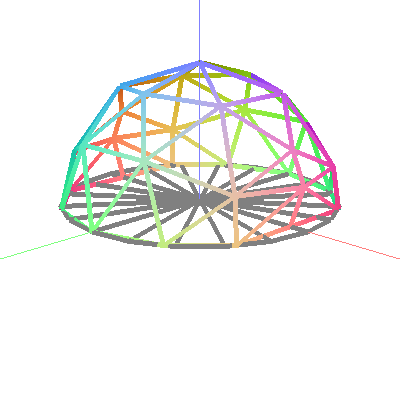
\includegraphics[width=5cm]{Figures/halficosphere1.png} }}%
  \qquad
  \subfloat[Poloviční dvacetistěn, \(3\times\) rozdělené polygony \label{fig:halficasehedron3}]{{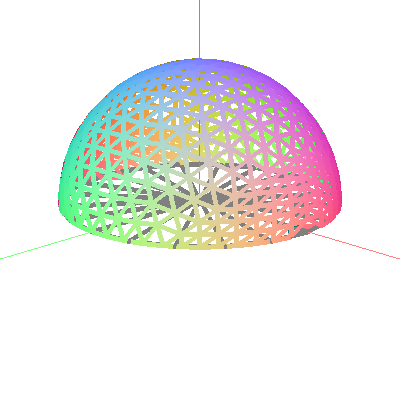
\includegraphics[width=5cm]{Figures/halficosphere3.png} }}%
  \caption{Postup generování hemisféry}%
  \label{fig:hemisfera}%
\end{figure}

Body takto generované hemisféry jsou následně upraveny ve vertex shaderu. Základní kód pro úpravu hemisféry glsl vertex shaderem je uveden ve \hyperref[src:vertexbrdf]{výpise \ref{src:vertexbrdf}}. Vertex shader pracuje se vstupními parametry \texttt{in\_Position}, \texttt{u\_incidentVector} a parametry pro jednotlivé BRDF funkce. Pro jednoduchost je výpis zkrácen a zjednodušen. Parametr \texttt{in\_Position} určuje vstupní bod hemisféry a před vstupem do brdf funkce je normalizován (aby byla pojištěna jednotková vzdálenost od středu). Parametr \texttt{u\_incidentVector} představuje směrový vektor $\outVec$. \par

\begin{listing}[ht]
  \inputminted{c++}{sampleshader.glsl}
  \caption{Zjednodušený vertex shader}
  \label{src:vertexbrdf}
\end{listing}

Ve vertex shaderu jsou poté ve funkci \texttt{BRDF()} implementovány jednotlivé BRDF funkce. Pro přepínání mezi aktuálně zvolenou BRDF funkcí slouží uniformní proměnná, která je do shaderu předávána z programu. Parametry jednotlivých funkcí jsou také předávány pomocí uniformních proměnných. Po zpracování ve vertex shaderu je následně vizualizace zpracována fragment shaderem, kde je každý bod vizualizace jednoduše obarven podle vzdálenosti bodu od středu (tzn. dle hodoty BRDF funkce daného bodu). Obarvení dané hodnoty BRDF funkce je provedeno za pomocí sekvenční barevné mapy \textit{YLGnBu}. Ukázka výsledné vizualizace je zobrazena na \hyperref[fig:brdfExample]{obrázku \ref{fig:brdfExample}}, kde je vizualizována fyzikálně korektní Phongova BRDF funkce.

\begin{figure}
  \centering
  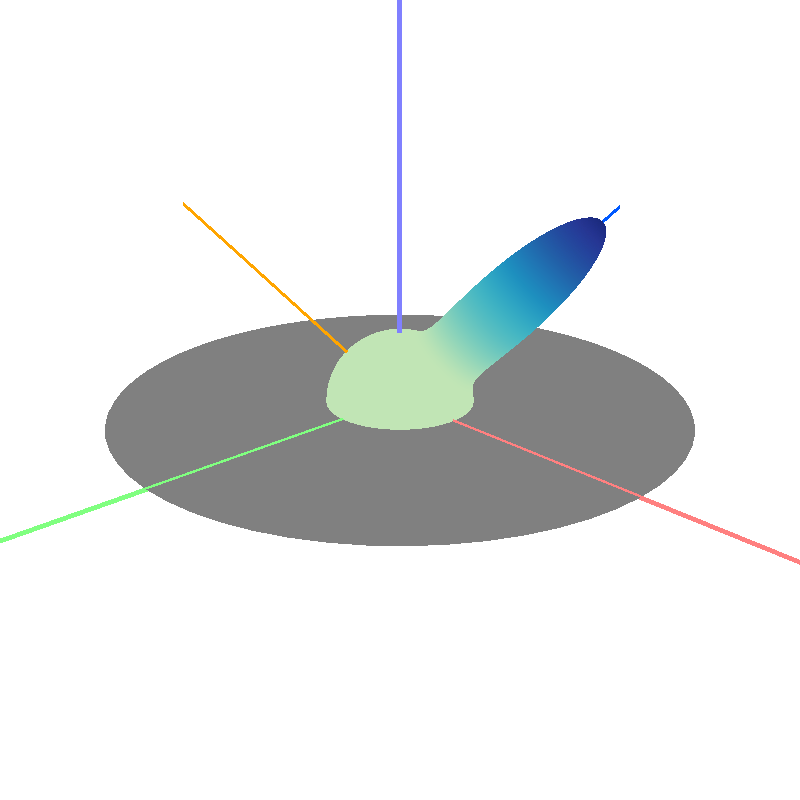
\includegraphics[width=6cm]{Figures/brdfVizExample.png}
  \caption{Ukázka vizualizace BRDF}%
  \label{fig:brdfExample}%
\end{figure}

\subsection{Vizualizace vzorkování}
Každou BRDF funkci je vhodné kombinovat s vhodně zvolenou vzorkovací funkci. Vzorkovací funkce jsou podrobněji popsány v kapitole \hyperref[sec:reduction]{\ref{sec:reduction} Redukce variance, optimalizace Monte carlo}. K vizualizaci vzorkovacích funkcí jsem se rozhodl přistoupit pomocí vizualizace vektory. Princip je v zásadě jednoduchý. Vzorkovací funkce pracují tak, že se vygeneruje směr pro náhodně vygenerované hodnoty $\randU$ a $\randV$. Vizualizace potom funguje na principu vygenerování uniformně rozložených hodnot v mřížce s daným rozlišením. Takto generované hodnoty jsou poté převedeny pomocí vzorkovací funkce do vektorů. Uniformně rozložené generované vektory jsou poté přímo zobrazeny. V případě potřeby je možné interaktivně zvýšit nebo snížit počet vzorků. Ve výchozím nastavení je délka jednotlivých vizualizovaných vektorů jednotková. Je také možné nastavit násobení velikostí vektorů hodnotou pdf. Na \hyperref[fig:samplingExample]{obrázku \ref{fig:samplingExample}} je zobrazena ukázka vizualizace vzorkovací funkce.

\begin{figure}
  \centering
  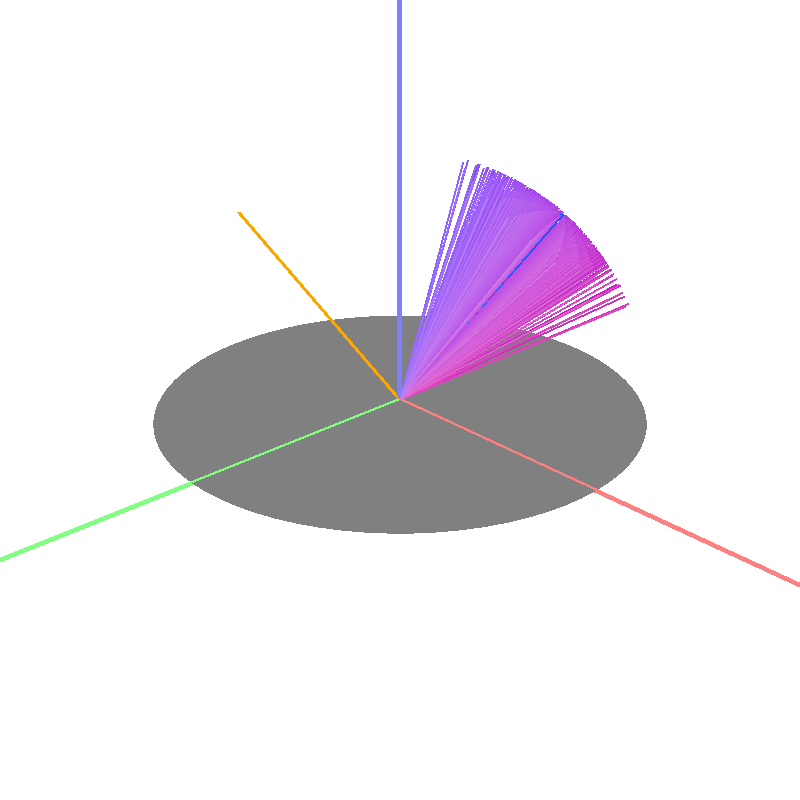
\includegraphics[width=6cm]{Figures/samplingExample.png}
  \caption{Ukázka vizualizace vzorkování}%
  \label{fig:samplingExample}%
\end{figure}


\subsection{Vizualizace výsledného renderu}

\clearpage
\section{Vybrané matematické funkce}

\subsection{Převod vektoru z lokálního do globálního prostoru}
V následujících kapitole \hyperref[sec:reduction]{\ref{sec:reduction} Redukce variance, optimalizace Monte carlo} jsou popsány metody generování vzorků vektorů používaných pro výpočet odrazu světla. Problémem ale je, že tyto generované vektory nejsou orientovány podél normály. Generované vektory jsou typicky orientovány podle $\uvec{up}$ vektoru (vektor určující ve scéně osu směrem nahoru). Pro použití s libovolnou normálou je tedy nutné výsledný vektor vygenerované vzorkovací funkcí orotovat podél normálového vektoru. Tato funkce má také využití např. při generování vzorků pro odrazovou složku Phongova BRDF (viz \hyperref[sec:phongSampling]{\ref{sec:phongSampling} Vzorkování Phongova BRDF}). Vzhledem k tomu, že vzorkovací funkce samotná je při renderingu volána velmi často, je vhodné mít všechny kroky vzorkování co nejlépe optimalizované. Jednou z nejlepších metod pro rotaci vektrou je použití transformační matice. Pro rotaci ve 3D prostoru se využívá trojice elementárních rotačních matic, definovaných \hyperref[eq:rotX]{vzorci \ref{eq:rotX}, \ref{eq:rotY} a \ref{eq:rotZ}} \cite{HughesDamEtAl13}\par
\begin{eqnarray}
  R_x(\theta) & = & \begin{bmatrix}
    1 & 0          & 0           \\
    0 & \cos\theta & -\sin\theta \\
    0 & \sin\theta & \cos\theta
  \end{bmatrix} \label{eq:rotX} \\
  R_y(\theta) & = & \begin{bmatrix}
    \cos\theta  & 0 & \sin\theta \\
    0           & 1 & 0          \\
    -\sin\theta & 0 & \cos\theta
  \end{bmatrix} \label{eq:rotY} \\
  R_z(\theta) & = & \begin{bmatrix}
    \cos\theta & -\sin\theta & 0 \\
    \sin\theta & \cos\theta  & 0 \\
    0          & 0           & 1
  \end{bmatrix}\label{eq:rotZ}
\end{eqnarray}
Cílem je získání rotační matice pro rotaci vektoru $\fromVect$ na vektor $\toVect$. Po aplikaci rotační matice na vygenerované vektory vzorkovacími funkcemi je dosaženo správné orientace vzorkovaných vektorů.  Efektivní výpočet rotační matice bez použití goniometrických funkcích je definován \hyperref[eq:vectRotation]{vzorcem \ref{eq:vectRotation}} \cite{MollerHughesVectRotation}.
\begin{equation} \label{eq:vectRotation}
  \begin{bmatrix}
    u_x^2 + \left ( 1 - u_x^2\right ) \cos\theta                & u_x u_y \left ( 1 - \cos \theta \right ) - y_z \sin \theta & u_x u_z + u_y \sin \theta                                  \\
    u_x u_y \left ( 1 -  \cos \theta \right ) + u_z \sin \theta & u_y^2 + \left ( 1 - u_y^2\right ) \cos\theta               & u_y u_z \left ( 1 - \cos \theta \right ) - u_x \sin \theta \\
    u_x u_z \left ( 1 - \cos \theta \right ) - u_y \sin \theta  & u_y u_z \left ( 1 - \cos \theta \right ) + u_x \sin \theta & u_z^2 + \left ( 1 - u_z^2\right ) \cos\theta
  \end{bmatrix}
\end{equation}
Pro výpočet se používá parametr $u$, což je normalizovaný vektor kolmý na vektory $\fromVect$ a $\toVect$. Z rovnice je také možné odstranit výpočet goniometrických funkcí, vzhledem k tomu, že platí: $\cos \theta = \fromVect \cdot \toVect$ a $\sin \theta = \left\Vert \fromVect \times \toVect \right\Vert$. Dále je možné zjednodušit výpočet pomocí substitucí \hyperref[eq:subst]{\ref{eq:subst}} na \hyperref[eq:vectRotationSimple]{vzorec \ref{eq:vectRotationSimple}} \cite{MollerHughesVectRotation}.

\begin{eqnarray} \label{eq:subst}
  c &=& \fromVect \cdot \toVect \nonumber\\
  v &=& \fromVect \times \toVect \nonumber\\
  h &=& \frac{1 - c}{1 - c^2} = \frac{1 - c}{v \cdot v} \nonumber
\end{eqnarray}

\begin{equation} \label{eq:vectRotationSimple}
  R\left ( \fromVect, \toVect \right) = \begin{bmatrix}
    c + h v_x^2     & h v_x v_y - v_z & h v_x v_z + v_y \\
    h v_x v_y + v_z & c + h v_y^2     & h v_y v_z - v_x \\
    h v_x v_z - v_y & h v_y v_z + v_x & c + h v_z^2
  \end{bmatrix}
\end{equation}

\subsection{Převod sférických souřadnic}
Při výpočtu vzorkování se často počítá se sférickými souřadnicemi. Pro převod vektoru definovaného sférickými souřadnicemi do kartézských souřadnic je možné použít \hyperref[eq:sphericalToCartesian]{vzorec \ref{eq:sphericalToCartesian}}
\begin{eqnarray}
  x & = & \sin(\theta)\cos(\phi)\nonumber \\
  y & = & \sin(\theta)\sin(\phi)\nonumber \\
  z & = & \cos(\theta)\label{eq:sphericalToCartesian}
\end{eqnarray}
Zpětný převod normalizovaného vektoru z kartézských souřadnic je také možný, pomocí \hyperref[eq:cartesianToSpherical]{vzorce \ref{eq:cartesianToSpherical}}

\begin{eqnarray}
  \theta & = & \arctan \frac{\sqrt{x^2 + y^2}}{z} \nonumber \\
  \phi & = & \arctan \frac{y}{x}\label{eq:cartesianToSpherical}
\end{eqnarray}

\clearpage
\section{Redukce variance, optimalizace Monte carlo} \label{sec:reduction}
Následující kapitoly se zabývají redukcí variance při výpočtu renderovací rovnice pomocí Monte Carlo metody.

\subsection{Vzorkování směrů odražených paprsků}

\subsection{Vzorkování hemisféry} \label{sec:hemisphere}
Jednou z nejjednodušších metod pro vzorkování je vzorkování hemisféry. Uniformní vzorkování hemisféry je definováno \hyperref[eq:hemisphereSampling]{vzorcem \ref{eq:hemisphereSampling}} (ve sférických souřadnicích). Rozdělení pravděpodobnosti je konstantní, definováno \hyperref[eq:hemisphereSamplingPdf]{vzorcem \ref{eq:hemisphereSamplingPdf}}. Při tomto vzorkování jsou všechny paprsky rovnoměrně rozdělené, všechny směry mají stejnou pravděpodobnost odrazu. Takové vzorkování je možné použít pro všechny BRDF funkce. Nevýhodou tohoto vzorkování je ale neoptimálnost vůči různým BRDF funkcím. Ideálně by vzorkovací funkce měla co nejpřesněji kopírovat BRDF funkci. \par

\begin{eqnarray}
  \theta & = & \arccos(\randU) \nonumber \\
  \phi & = & 2\pi\randV \label{eq:hemisphereSampling}
\end{eqnarray}

\begin{equation} \label{eq:hemisphereSamplingPdf}
  p = \frac{1}{2\pi}
\end{equation}

Jedna z možností optimalizace je použití vzorkování hemisféry závislém na cosinu úhlu mezi vstupním paprskem a normálou povrchu. Základní tezí je, že paprsky s největším úhlem mají nejmenší vliv na výsledné osvětlení v daném bodě. Vzorkování by tedy mělo mít rozložení vzorků více kumulované ve směru normály oproti ostatním směrům. Jednou z možností jak generovat paprsky touto metodou je pomocí Malleyho metody. Tato metoda spočívá v generování bodu v jednotkovém disku pomocí soustředných kruhů \cite{PHARR2017747}. Výsledné souřadnice v kartézském systému se vypočítají pomocí \hyperref[eq:concentricHemisphere]{vzorce \ref{eq:concentricHemisphere}}. Pro výpočet je potřeba převést $\randU$ a $\randV$ z intervalu $\interval{0;1}$ do intervalu $\interval{-1;1}$  Rozdělení pravděpodobnosti je definováno \hyperref[eq:concentricHemisphere]{vzorcem \ref{eq:concentricHemispherePdf}}.

\begin{eqnarray}
  r & = & \left\{\begin{matrix*}[l] \randU & |\randU| > \left | \randV \right |\\ \randV & jinak \end{matrix*}\right. \nonumber \\
  \Theta & = & \left\{\begin{matrix*}[l] \frac{\pi}{4}\frac{\randV}{\randU} & |\randU| > \left | \randV \right |\\ \frac{\pi}{2}-\frac{\pi}{4}\frac{\randU}{\randV} & jinak \end{matrix*}\right. \nonumber \\
  x & = &r\cos(\Theta)\nonumber \\
  y & = &r\sin(\Theta)\nonumber \\
  z & = &\sqrt{ \max(0, 1 - x^2 + y^2) }\label{eq:concentricHemisphere}
\end{eqnarray}

\begin{equation} \label{eq:concentricHemispherePdf}
  p = \frac{\cos\theta}{\pi}
\end{equation}

\subsection{Vzorkování Phongova BRDF} \label{sec:phongSampling}
Pro vzorkování Phongova BRDF je potřeba rozhodnout, kterou část BRDF vzorkujeme - jestli difuzivní nebo odrazovou. Toto rozhodnutí je možné vytvořit náhodně, pomocí vygenerování náhodného čísla $\xi$ z intervalu $\interval{0;k_d+k_s}$. Pokud $\xi < k_d$, je vzorkována difuzivní část. V opačném případě je vzorkována odrazová část \cite{KrivanekBRDFIBL}.
\subsubsection{Vzorkování difuzivní části}
Difuzivní část je možné vzorkovat pomocí \hyperref[sec:hemisphere]{hemisféry (\ref{sec:hemisphere})}. Je možné také použít hemisféru závislou na cosinu úhlu mezi vstupním paprskem a normálou povrchu.

\subsubsection{Vzorkování odrazové části}
Pro vzorkování odrazové části je vzorkován phongův cosinový lalok, který je vycentrován okolo $\refl$. Výpočet vzorkování odrazové části je definován \hyperref[eq:phongSpecularSample]{vzorcem \ref{eq:phongSpecularSample}} \cite{KrivanekBRDFIBL}. Rozdělení pravděpodobnost je definováno \hyperref[eq:phongSpecularSamplePdf]{vzorcem \ref{eq:phongSpecularSamplePdf}}.
Výsledek tohoto vzorkování je vycentrován okolo normály, je tedy potřeba rotovat výsledek podél $\refl$. K rotaci vektoru je možné využít \hyperref[eq:vectRotationSimple]{vzorec \ref{eq:vectRotationSimple}}.

\begin{eqnarray}
  \theta & = & \arccos(\randU^{\frac{1}{n+1}}) \nonumber \\
  \phi & = & 2\pi\randV\label{eq:phongSpecularSample}
\end{eqnarray}

\begin{equation} \label{eq:phongSpecularSamplePdf}
  p = \frac{n+1}{2\pi}\cos^n\theta
\end{equation}

\subsubsection{Výsledné vzorkování}
Po spojení vzorkování odrazové a difuzivní části je vhodné adaptovat i výpočet samotného BRDF. Při vzorkování difuzivní části je třeba jako BRDF funkci použít pouze difuzivní část Phongova BRDF, při vzorkování odrazové části je použita odrazová část Phongova BRDF. Pokud by se použilo Phongovo BRDF bez úpravy, nebylo by dosaženo snížení variance ve výsledném obrazu. \cite{KrivanekBRDFIBL}

\printbibliography[title={Literatura}, heading=bibintoc]

\appendix
\section{Užité symboly}

\subsection{Obecné}

\begin{itemize}
  \item[\(\outRadiance\):] Výsledná zář vyzařovaná z daného bodu
  \item[\(\emitRadiance\):] Zář, pasivně vyzařovaná z objektu v daném bodě
  \item[\(\inRadiance\):] Zář dopadající na daný bod
  \item[\(\irradiance\):] Celková žář dopadající na daný bod
  \item[\(\brdf\):] BRDF funkce
  \item[\(\left(\theta,\phi\right)\):] Vektor definovaný sférickými souřadnicemi
  \item[\(\left(x,y,z\right)\):] Vektor definovaný kartézskými souřadnicemi
  \item[\(\normVec\):] Vektor normály povrchu
  \item[\(\inVec\):] Vektor ve směru ke světelnému zdroji. Platí: \(\inVec = \left(\theta_i,\phi_i\right)\)
  \item[\(\outVec\):] Vektor ve směru k pozorovateli. Platí: \(\outVec = \left(\theta_o,\phi_o\right)\)
  \item[\(\refl\):] Vektor zrcadlového odrazu světla, platí: \(\refl = 2\left(\inVec\cdot\normVec\right)\normVec-\inVec\)
  \item[\(\halfVec\):] Poloviční vektor mezi pohledovým a světelným vektorem. Platí: \(\halfVec = \frac{\inVec + \outVec}{\| \inVec + \outVec\|}\)
  \item[\(\theta_r\):] Úhel odrazu, platí: \(\cos\theta_r = \outVec\cdot\refl\)
\end{itemize}

\subsection{Vzorkování}

\begin{itemize}
  \item[\(\randU\):] Náhodné číslo $\in \mathbb{R}, \interval{0,1}$
  \item[\(\randV\):] Náhodné číslo $\in \mathbb{R}, \interval{0,1}$
\end{itemize}

\subsection{BRDF}

\begin{itemize}
  \item[\(\alb\):] Albedo materiálu, poměr mezi pohlceným a odraženým světlem (Lambert)
  \item[\(k_s\):] Koeficient odrazivosti materiálu (Phong)
  \item[\(k_d\):] Koeficient difuze materiálu (Phong)
  \item[\(n\):] Koeficient lesklosti materiálu (Phong)
  \item[\(\rough\):] Koeficient drsnosti povrchu - roughness(Torrance-Sparrow, Cook-Torrance, Oren-Nayar)
  \item[\(\ior\):] Koeficient lomu světla - ior (Torrance-Sparrow, Cook-Torrance)
\end{itemize}

\end{document}